\section{Event Distributions for Optimized FV cuts}
\label{sec:evtdist}

%This section shows the distributions of the reconstructed \wall, \towall and neutrino energy
%for various signal and background channels.  

%% NUE %%%%%%%%%%%%%%%%%%%%%%%%%%%%%%%%%%%%%%%%%%%%%%%%
\begin{figure}[h]
  \begin{center}
    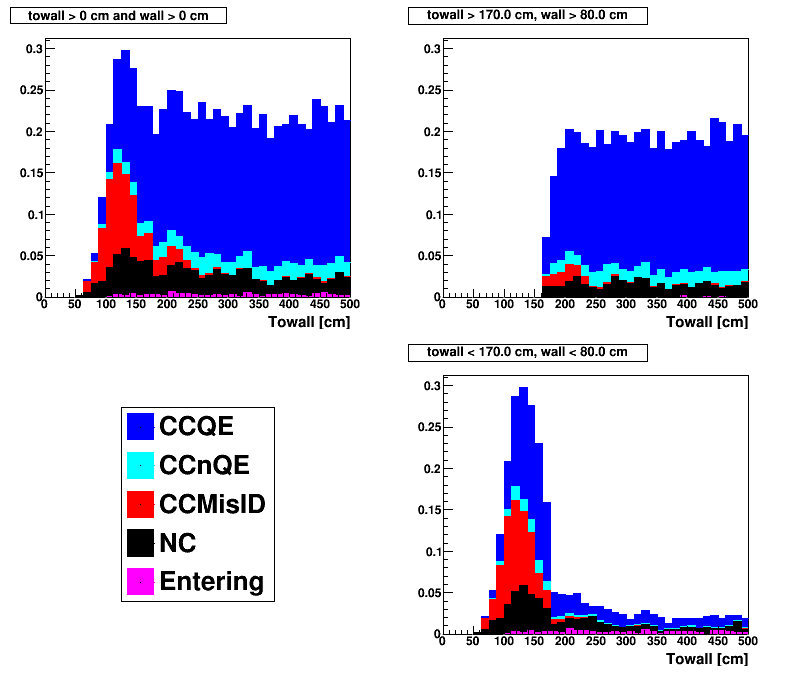
\includegraphics[width=0.9\textwidth]{tw170_nue__towall_}
  \end{center}
  \caption{Plots of the various MC categories that pass the T2K \nue
  topological cuts binned in reconstructed \towall in various detector regions. Upper left
  plot shows the distribution for only fully-contained cuts (i.e. FV cut is \@ $wall > 0$ cm).
  Upper right plot shows the distribution for the optimized FV cut for this selction.
  Lower Right plot shows the distribution of the events \emph{rejected} by the optimized
  FV cuts for this sample.
  }
  \label{fig:compnuetowall}
\end{figure}


\begin{figure}[h]
  \begin{center}
    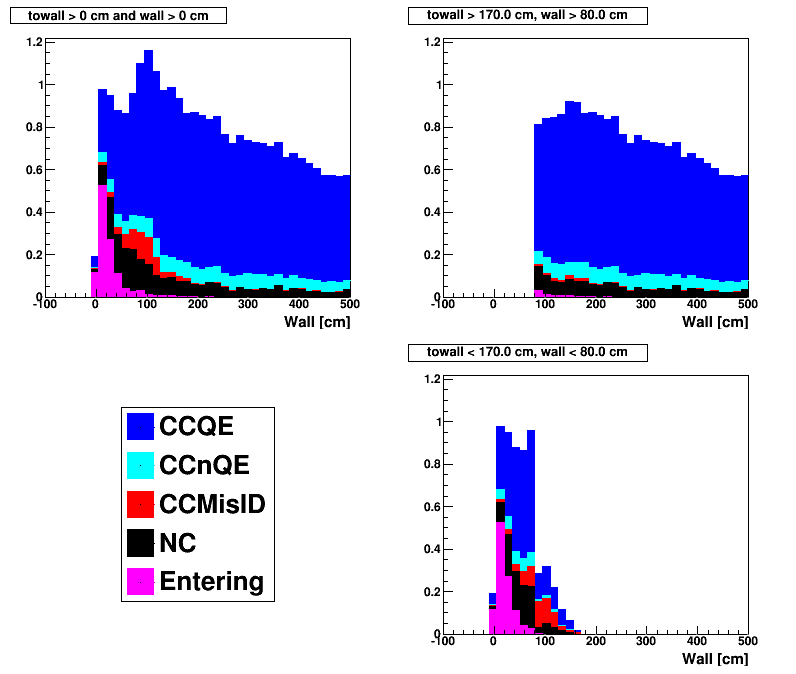
\includegraphics[width=0.9\textwidth]{tw170_nue__wall_}
  \end{center}
  \caption{Plots of the various MC categories that pass the T2K \nue
  topological cuts binned in reconstructed \wall in various detector regions. Upper left
  plot shows the distribution for only fully-contained cuts (i.e. FV cut is \@ $wall > 0$ cm).
  Upper right plot shows the distribution for the optimized FV cut for this selction.
  Lower Right plot shows the distribution of the events \emph{rejected} by the optimized
  FV cuts for this sample.
  }
  \label{fig:compnuewall}
\end{figure}


\begin{figure}[h]
  \begin{center}
    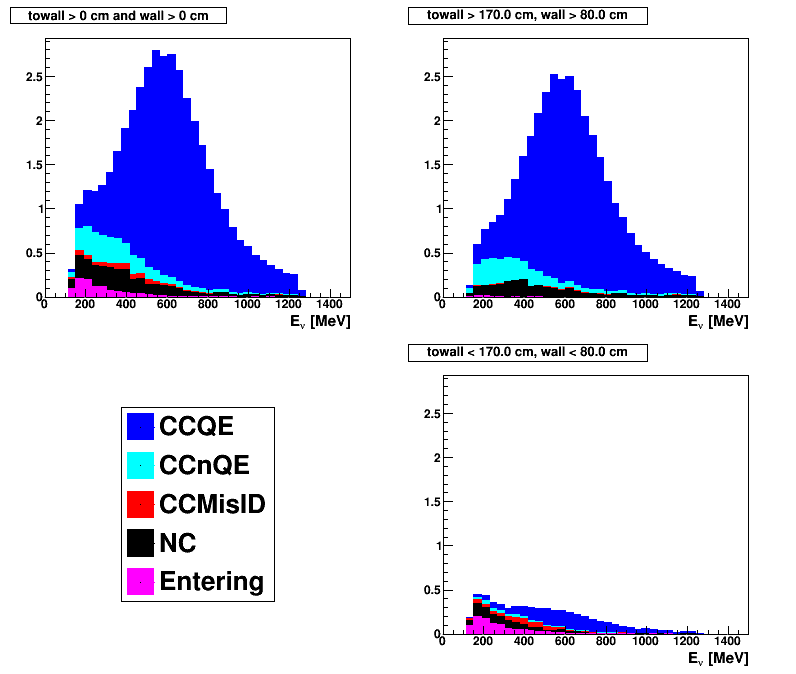
\includegraphics[width=0.9\textwidth]{tw170_nue__erec_}
  \end{center}
  \caption{Plots of the various MC categories that pass the T2K \nue
  topological cuts binned in reconstructed neutrino energy in various detector
  regions. Upper left plot shows the distribution for only fully-contained cuts
  (i.e. FV cut is \@ $wall > 0$ cm).  Upper right plot shows the distribution
  for the optimized FV cut for this selction.  Lower Right plot shows the
  distribution of the events \emph{rejected} by the optimized FV cuts for this
  sample.
  }
  \label{fig:compnueerec}
\end{figure}

%% NUMU %%%%%%%%%%%%%%%%%%%%%%%%%%%%%%%%%%%%%%%%%%%%%%%%
\begin{figure}[h]
  \begin{center}
    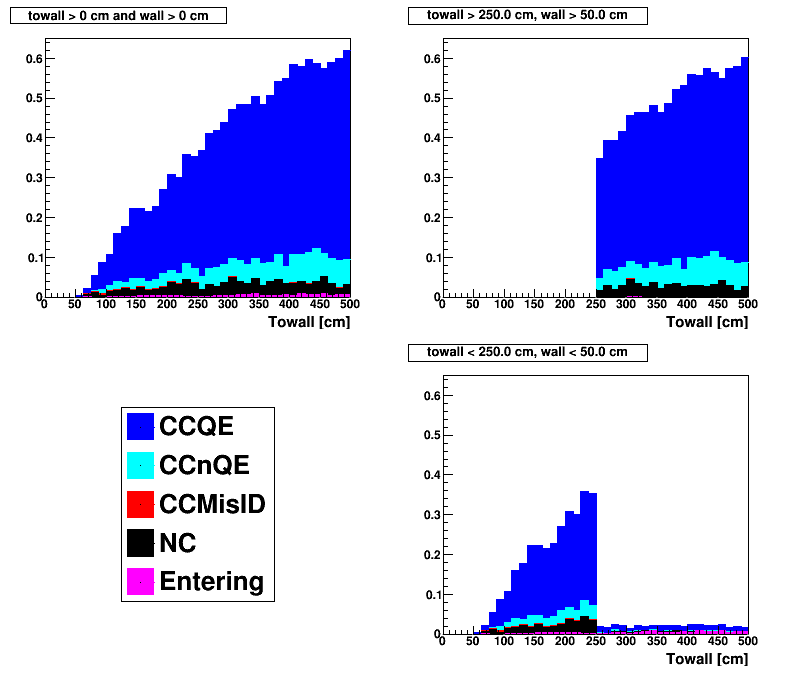
\includegraphics[width=0.9\textwidth]{tw250_numu__towall_}
  \end{center}
  \caption{Plots of the various MC categories that pass the T2K \numu
  topological cuts binned in reconstructed \towall in various detector regions. Upper left
  plot shows the distribution for only fully-contained cuts (i.e. FV cut is \@ $wall > 0$ cm).
  Upper right plot shows the distribution for the optimized FV cut for this selction.
  Lower Right plot shows the distribution of the events \emph{rejected} by the optimized
  FV cuts for this sample.
  }
  \label{fig:compnumutowall}
\end{figure}


\begin{figure}[h]
  \begin{center}
    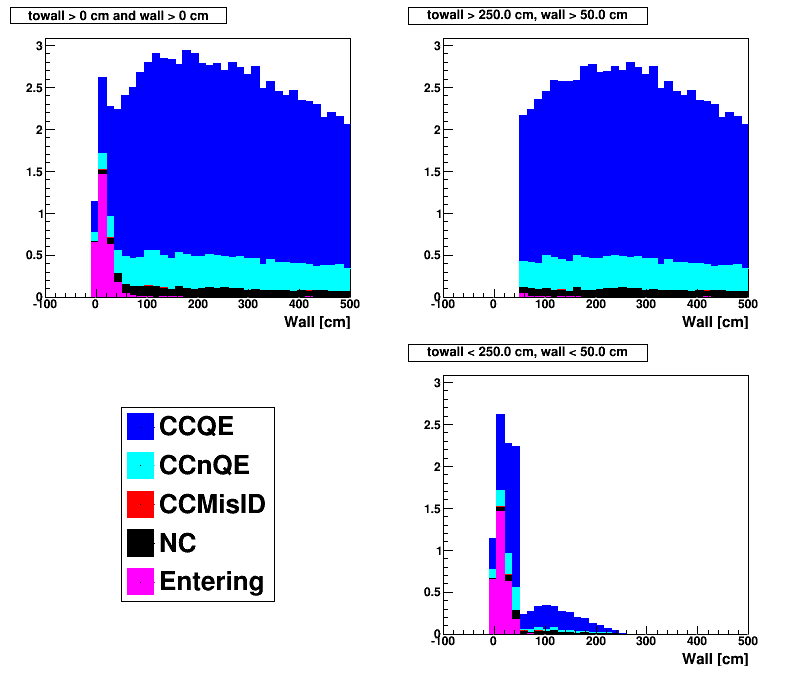
\includegraphics[width=0.9\textwidth]{tw250_numu__wall_}
  \end{center}
  \caption{Plots of the various MC categories that pass the T2K \numu
  topological cuts binned in reconstructed \wall in various detector regions. Upper left
  plot shows the distribution for only fully-contained cuts (i.e. FV cut is \@ $wall > 0$ cm).
  Upper right plot shows the distribution for the optimized FV cut for this selction.
  Lower Right plot shows the distribution of the events \emph{rejected} by the optimized
  FV cuts for this sample.
  }
  \label{fig:compnumuwall}
\end{figure}


\begin{figure}[h]
  \begin{center}
    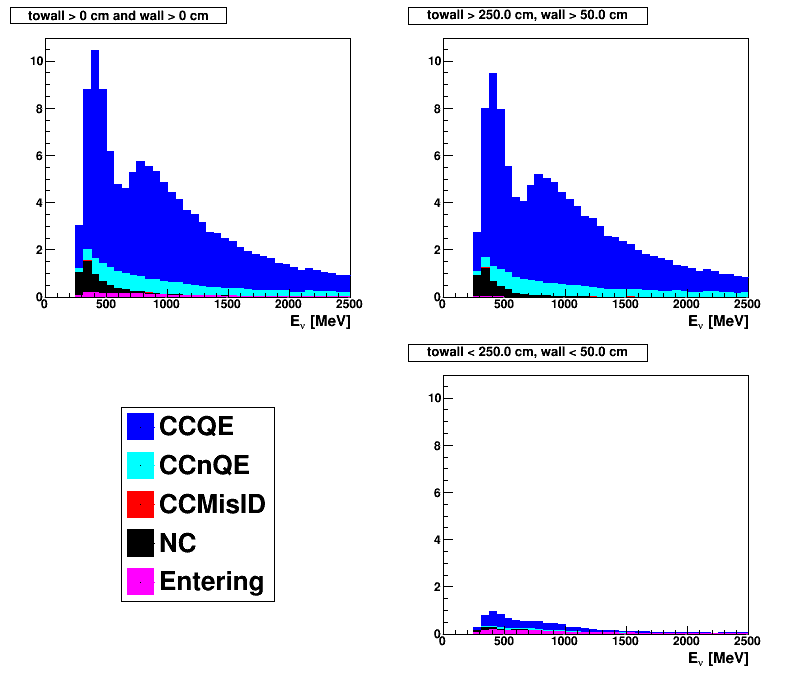
\includegraphics[width=0.9\textwidth]{tw250_numu__erec_}
  \end{center}
  \caption{Plots of the various MC categories that pass the T2K \numu
  topological cuts binned in reconstructed neutrino energy in various detector
  regions. Upper left plot shows the distribution for only fully-contained cuts
  (i.e. FV cut is \@ $wall > 0$ cm).  Upper right plot shows the distribution
  for the optimized FV cut for this selction.  Lower Right plot shows the
  distribution of the events \emph{rejected} by the optimized FV cuts for this
  sample.
  }
  \label{fig:compnumuerec}
\end{figure}


%% NUE1RPI %%%%%%%%%%%%%%%%%%%%%%%%%%%%%%%%%%%%%%%%%%%%%%%%
\begin{figure}[h]
  \begin{center}
    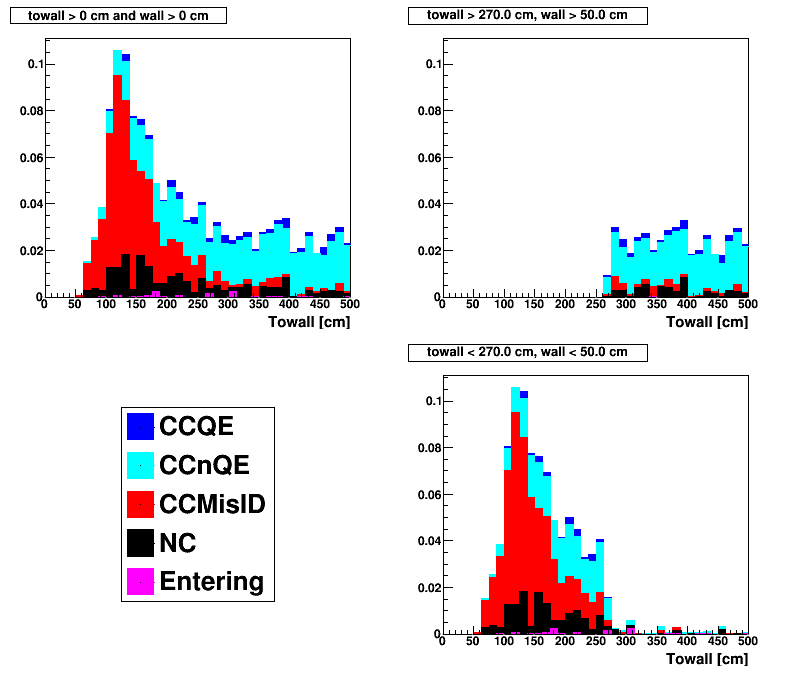
\includegraphics[width=0.9\textwidth]{tw270_nue1rpi__towall_}
  \end{center}
  \caption{Plots of the various MC categories that pass the T2K  \nue CC1R$pi$
  topological cuts binned in reconstructed \towall in various detector regions. Upper left
  plot shows the distribution for only fully-contained cuts (i.e. FV cut is \@ $wall > 0$ cm).
  Upper right plot shows the distribution for the optimized FV cut for this selction.
  Lower Right plot shows the distribution of the events \emph{rejected} by the optimized
  FV cuts for this sample.
  }
  \label{fig:compnue1rpitowall}
\end{figure}


\begin{figure}[h]
  \begin{center}
    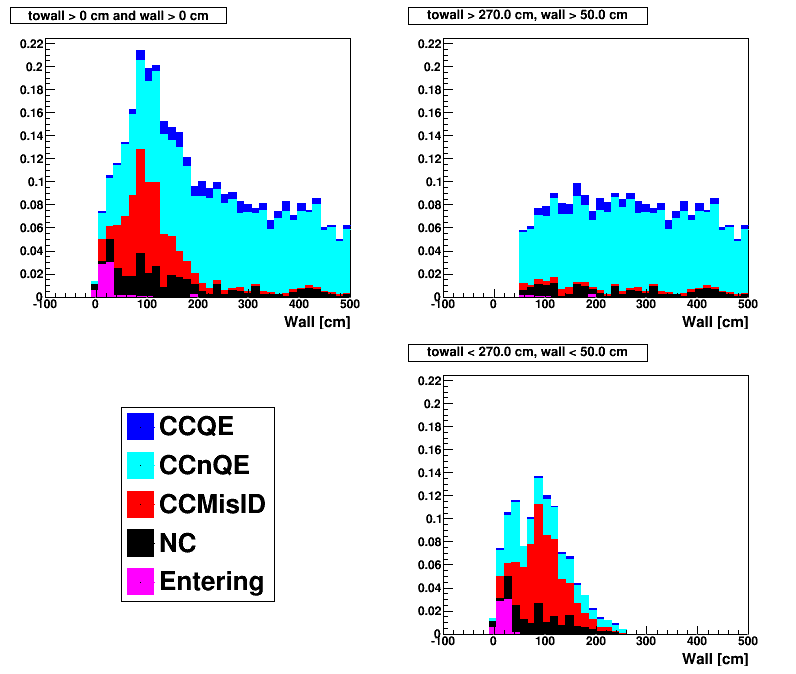
\includegraphics[width=0.9\textwidth]{tw270_nue1rpi__wall_}
  \end{center}
  \caption{Plots of the various MC categories that pass the T2K \nue CC1R$pi$
  topological cuts binned in reconstructed \wall in various detector regions. Upper left plot
  shows the distribution for only fully-contained cuts (i.e. FV cut is \@ $wall
  > 0$ cm).  Upper right plot shows the distribution for the optimized FV cut
  for this selction.  Lower Right plot shows the distribution of the events
  \emph{rejected} by the optimized FV cuts for this sample.
  }
  \label{fig:compnue1rpiwall}
\end{figure}


\begin{figure}[h]
  \begin{center}
    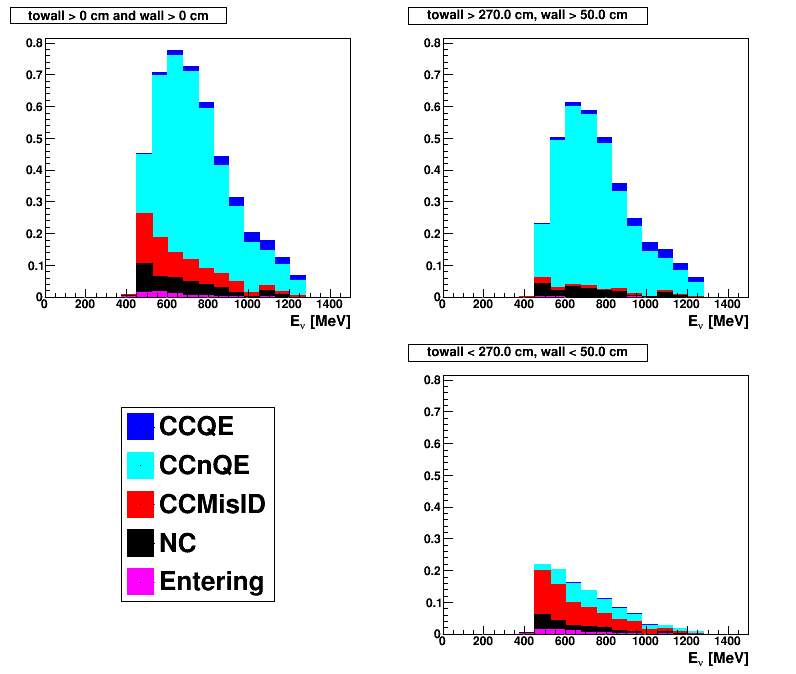
\includegraphics[width=0.9\textwidth]{tw270_nue1rpi__erec_}
  \end{center}
  \caption{Plots of the various MC categories that pass the T2K \nue CC1R$pi$
  topological cuts binned in reconstructed neutrino energy in various detector
  regions. Upper left plot shows the distribution for only fully-contained cuts
  (i.e. FV cut is \@ $wall > 0$ cm).  Upper right plot shows the distribution
  for the optimized FV cut for this selction.  Lower Right plot shows the
  distribution of the events \emph{rejected} by the optimized FV cuts for this
  sample.
  }
  \label{fig:compnue1rpierec}
\end{figure}

